\documentclass[12pt]{standalone}
\usepackage{tikz}
\usetikzlibrary{decorations.pathreplacing}
\usetikzlibrary{decorations.markings}
\usetikzlibrary{positioning}
\usetikzlibrary{shapes}

\usetikzlibrary{backgrounds}

\begin{document}
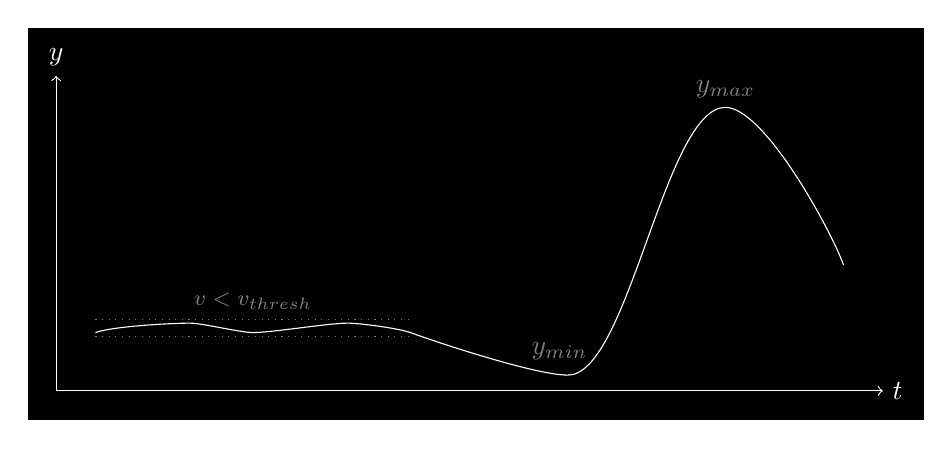
\begin{tikzpicture}
	[scale=10,
	color=white,
	background rectangle/.style={fill=black},
	show background rectangle]

\IfStandalone {\tikzstyle{subtle}=[thin,gray]
\tikzstyle{subtle line}=[thin,gray!60]} {\tikzstyle{subtle}=[thin,gray]
\tikzstyle{subtle line}=[thin,gray!60]}

\def\XOffset{-0.05}
\def\TickLength{0.01}
\def\SafetyMargin{0.005}

\def\TotalHeight{0.4}
\pgfmathsetmacro{\StillCenter}{0.2 * \TotalHeight}
\def\StillThresh{0.006}
\pgfmathsetmacro{\StillTop}{\StillCenter + \StillThresh}
\pgfmathsetmacro{\StillBottom}{\StillCenter - \StillThresh}

\pgfmathsetmacro{\MotionBottom}{0.05 * \TotalHeight}
\pgfmathsetmacro{\MotionTop}{0.9 * \TotalHeight}

\pgfmathsetmacro{\MotionEnd}{0.4 * \TotalHeight}

\def\StillEnd{0.4}
\def\BottomTime{0.6}
\def\TopTime{0.8}
\def\EndTime{0.95}

% Axes
\draw [<->]
	(\XOffset, \TotalHeight) node (yaxis) [above] {$y$} |-
	(1, 0) node (xaxis) [right] {$t$};

% Still threshold indicators
\draw[subtle, dotted]
	(0, \StillBottom - \SafetyMargin) --
	(\StillEnd, \StillBottom - \SafetyMargin);
\draw[subtle, dotted]
	(0, \StillTop + \SafetyMargin) --
	(\StillEnd, \StillTop + \SafetyMargin)
	node [midway, above, subtle] {\footnotesize $v < v_{thresh}$};

%\draw
%	(\XOffset - 0.5 * \TickLength, \StillBottom - \SafetyMargin) --
%	(\XOffset + 0.5 * \TickLength, \StillBottom - \SafetyMargin);
%\draw
%	(\XOffset - 0.5 * \TickLength, \StillTop + \SafetyMargin) --
%	(\XOffset + 0.5 * \TickLength, \StillTop + \SafetyMargin);
%\path (\XOffset, \StillBottom) -- (\XOffset, \StillTop)
%	node [black,midway,left] {$\Delta y_i$};

% Motion amplitude indicators
%\draw[subtle line]
%	(\BottomTime, \MotionBottom) --
%	(\EndTime, \MotionBottom);
%\draw[subtle line]
%	(\TopTime, \MotionTop) --
%	(\EndTime, \MotionTop);
%\draw [decorate,decoration={brace,mirror,amplitude=4pt,raise=1pt}]
%	(\EndTime, \MotionBottom) -- (\EndTime, \MotionTop)
%	node [black,midway,xshift=0.6cm] {$\Delta y_g$};

% Still time indicators
%\draw
%	(0, 0.5 * \TickLength) --
%	(0, -0.5 * \TickLength);
%\draw
%	(\StillEnd, 0.5 * \TickLength) --
%	(\StillEnd, -0.5 * \TickLength);
%\draw
%	[decorate,decoration={brace,mirror,amplitude=4pt,raise=1pt}]
%	(0, -\TickLength) -- (\StillEnd, -\TickLength)
%	node [black,midway,below,yshift=-6pt] {$\Delta t_i$};

% Gesture time indicators
%\draw [subtle line]
%	(\BottomTime, \MotionBottom) --
%	(\BottomTime, 0);
%\draw [subtle line]
%	(\TopTime, \MotionTop) --
%	(\TopTime, 0);
%\draw
%	(\BottomTime, 0.5 * \TickLength) --
%	+(0, -\TickLength);
%\draw
%	(\TopTime, 0.5 * \TickLength) --
%	+(0, -\TickLength);
%\draw
%	[decorate,decoration={brace,mirror,amplitude=4pt,raise=1pt}]
%	(\BottomTime, -\TickLength) -- (\TopTime, -\TickLength)
%	node [black,midway,below,yshift=-6pt] {$\Delta t_g$};

% Motion line
\draw[looseness=0.5]
	(0.0 * \StillEnd, \StillBottom) to[out=20,in=180]
	(0.3 * \StillEnd, \StillTop) to[out=0,in=180]
	(0.5 * \StillEnd, \StillBottom) to[out=0,in=180]
	(0.8 * \StillEnd, \StillTop) to[out=0,in=160]
	(1.0 * \StillEnd, \StillBottom) to[out=-20,in=180]
	(\BottomTime, \MotionBottom)
	node[above,gray,yshift=2pt,xshift=-3pt] {$y_{min}$} to[out=0,in=180]
	(\TopTime, \MotionTop) node[above,gray] {$y_{max}$} to[out=0,in=110]
	(\EndTime, \MotionEnd);
	
\end{tikzpicture}
\end{document}